% !TeX program = lualatex -synctex=1 -interaction=nonstopmode --shell-escape %.tex

\documentclass[12pt, table]{exam}
\usepackage[rus]{borochkin}

\usepackage{borochkin_exam_eng}

%%%%%%%%%%%%%%%%%%%%%%%%%%%%%%%%%%%%%%%%%

\professor
\iftagged{professor}{ \printanswers }

%%%%%%%%%%%%%%%%%%%%%%%%%%%%%%%%%%%%%%%%%


\begin{document}
\setcounter{section}{0\relax}%
\noindent
% Control № #1, Variant #2, Subject #3
\studentpersonalinfo{1}{2}{IF}
\normalsize

\begin{questions}
	\question[40] Test
	\answerstotestShort
	
	\question[20] The table below shows how the USDRUB exchange rate fluctuated from 01.11.2014 to 01.11.2015. Option expiration date is 01.01.2016 (option term is 2 months). Option execution price is 75 roubles per 1 US dollar. The USD risk free rate is 1\% annual, the RUB risk free rate is 8\% annual. Use binomial option pricing model as a methodology. 
	
	Evolution of USDRUB exchange rate during 01.11.2014 to 01.11.2015 period of time:
	\begin{table}[htbp]
		\centering
		\begin{tabular}{rr}
			\toprule
			Date & Exchange rate \\ \midrule
			11/1/2014 &       49.3837 \\
			12/1/2014 &       60.2065 \\
			1/1/2015 &       69.6717 \\
			2/1/2015 &       61.7096 \\
			3/1/2015 &         58.09 \\
			4/1/2015 &       51.4724 \\
			5/1/2015 &       52.2844 \\
			6/1/2015 &       55.1546 \\
			7/1/2015 &       61.3668 \\
			8/1/2015 &       64.2563 \\
			9/1/2015 &       65.3079 \\
			10/1/2015 &       63.4648 \\
			11/1/2015 &        66.061
		\end{tabular}%
	\end{table}
	
	
	\begin{subparts}
		\subpart[5] Calculate mean and standard deviation of currency rate monthly returns
		\begin{solution}[8em]
			
			m = 2.9080\%
			
			s = 10.1345\%	
		\end{solution}
		
		\subpart[10] Compute the call option price if the purchase is planned at 01.11.2015.
		\begin{solution}[20em]
			
			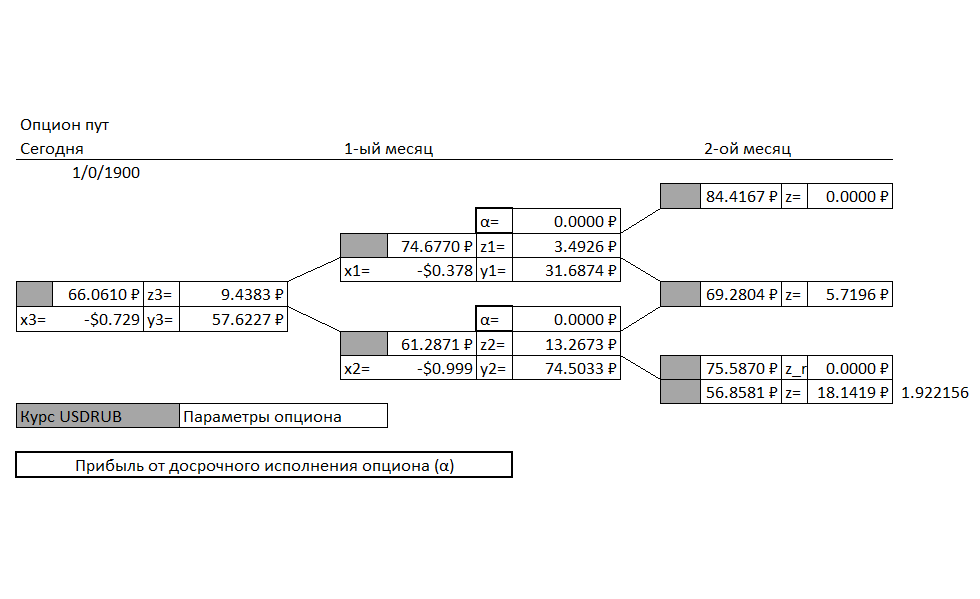
\includegraphics[height=8.5cm]{img/option_put_usdrub.png}
		\end{solution}
		
		\subpart[5] Suppose, the USDRUB exchange will reach 72,0633 at 01.12.2015 and 75,587 at 01.01.2016. How much profit would trader make if he invested 1000 USD in this financial instrument at 01.11.2015.
		\begin{solution}[8em]
			
			Option premium would be lost.
			
		\end{solution}
		
	\end{subparts}
	\addpoints
	
	\pagebreak
	\question[10] The Russian enterprise plans to attract 700 thousand rubles for 1 year. It has an opportunity to raise funds in rubles at the fixed rate of 16\% per annum and in euro at the fixed rate of 9\% per annum. A current EUR/RUB exchange rate is 47,00. What has to be EUR/RUB exchange rate at the period end so that the ruble cost of financial resources was identical in any case?
	
	\begin{solution}[8em]
		
		Loan, RUR.	700000
		
		Period, years	1
		
		Interest rate in RUR	16,00\%
		
		Interest rate in EUR	9,00\%
		
		RUR/EUR rate	47
		
		Demanded RUR/EUR rate	50,02
				
	\end{solution}
	
	\question[10] The company prepares a project. For this purpose it needs to attract 8.5 million rubles for the term of 1 year and 9 months. After the project end the company will be able to return to the creditor no more than 11 million rubles. The company has possibility to attract the loan in foreign currency. A current USD/RUR rate is 35,00. The loan must be repaid at the period end with interest. According to forecasts, in 1 year and 3 months USD/RUR rate will fluctuate between 36,00 to 39,00. What are the minimal and maximal acceptable interest rates of the loan?
	
	\begin{solution}[8em]
		
		Loan, mln RUR	8,5
		
		Period, years	1,75
		
		Loan limit, mln RUR	11
		
		Current RUR/USD rate	35
		
		Maximal forecasted RUR/USD rate	36
		
		Minimal forecasted RUR/USD rate	39
		
		Loan, mln USD	0,2429
		
		Maximal loan, mln USD	0,31
		
		Minimal loan, mln USD	0,28
		
		Maximal interest rate	14,75\%
		
		Minimal interest rate	9,22\%		
		
	\end{solution}
\end{questions}
\pagebreak
\noindent\textbf{Tests (choose one the most suitable answer)}

\begin{questions}
\begin{multicols}{2}
\setlength{\columnsep}{1cm}

\question During globalization the competition in domestic financial markets:
	 \begin{choices}
	 \CC increases;
	 \choice decreases;
	 \choice remains invariable;
	 \choice changes in an unpredictable way.
	 \end{choices}
\question During financial globalization grows by the greatest rates:
	 \begin{choices}
	 \choice equity market;
	 \CC bond market;
	 \choice credit market;
	 \choice market of financial derivatives.
	 \end{choices}
\question Characteristic feature of financial globalization is:
	 \begin{choices}
	 \choice increase of interest rates stability;
	 \choice growth of banking capital concentration;
	 \choice toughening the control of the international financial operations;
	 \CC increase in duration of the international financial operations.
	 \end{choices}
\question Increase of a country sovereign credit rating promotes:
	 \begin{choices}
	 \choice strengthening of the national financial market integration into the world;
	 \choice weakening of the national financial market integration into the world;
	 \choice the invariable level of the national financial market integration into the world;
	 \CC unpredictable changes of the level of the national financial market integration into the world.
	 \end{choices}
\question Financial derivatives are mostly used by:
	 \begin{choices}
	 \CC traders;
	 \choice arbitrageurs;
	 \choice intermediaries;
	 \choice hedgers.
	 \end{choices}
\question The international financial market open hours are:
	 \begin{choices}
	 \choice from 8 to 18 Coordinated Universal Time (UTC);
	 \choice from 6 to 20 UTC;
	 \CC from 4 to 22 UTC;
	 \choice round the clock.
	 \end{choices}
\question Speculative operations in the world financial market:
	 \begin{choices}
	 \CC increase its liquidity and price stability;
	 \choice reduce its liquidity and price stability;
	 \choice increase its liquidity and reduce price stability;
	 \choice reduce its liquidity and increase price stability.
	 \end{choices}
\question Role of institutional investors in functioning of the international financial market in the last decades:
	 \begin{choices}
	 \CC has been growing;
	 \choice has been decreasing;
	 \choice remained invariable;
	 \choice has been changing without a certain tendency.
	 \end{choices}
\question The international financial market is more profitable for:
	 \begin{choices}
	 \choice industrialized countries;
	 \CC developing countries — exporters of oil;
	 \choice developing countries — importers of oil;
	 \choice the countries with a transitional economy.
	 \end{choices}
\question Characteristic feature of modern international financial market is NOT:
	 \begin{choices}
	 \choice wide use of computer technologies of communication;
	 \CC high extent of financial instruments diversification;
	 \choice financial instruments quotes stability;
	 \choice high level of tax rates.
	 \end{choices}
\question Characteristic features of the modern world financial market are:
	 \begin{choices}
	 \choice large scale speculative operations;
	 \CC free capital movements between market segments;
	 \choice formation of the virtual capitals (financial bubbles);
	 \choice all above mentioned.
	 \end{choices}
\question Functions of the modern world financial market are:
	 \begin{choices}
	 \choice hedging of risks of the market participants;
	 \CC redistribution of world economy financial resources;
	 \choice formation of equilibrium level of interest rates, currency exchange rates and equities quotes;
	 \choice all above mentioned.
	 \end{choices}
\question Standardization of the contract terms is characteristic:
	 \begin{choices}
	 \choice for the futures foreign exchange market;
	 \choice over-the-counter Forex market;
	 \CC forward currency market;
	 \choice spot currency market.
	 \end{choices}
\question The market of foreign currency cash serves mainly:
	 \begin{choices}
	 \choice enterprises;
	 \choice financial institutions;
	 \CC government bodies;
	 \choice population.
	 \end{choices}
\question The cross rate is expressed:
	 \begin{choices}
	 \choice in the direct quotation;
	 \CC in the indirect quotation;
	 \choice both in the direct, and in the indirect quotation;
	 \choice in the specific quotation of a cross rate.
	 \end{choices}
\question The spread on less stable currency is equal A, the spread on stable currency is equal B In this case:
	 \begin{choices}
	 \choice A is more than B;
	 \CC A is less than B;
	 \choice A slightly differs from B;
	 \choice A differs in an unpredictable way from B.
	 \end{choices}
\question If external debt of Russia decreases, a ruble exchange rate to leading world currencies:
	 \begin{choices}
	 \CC will increase;
	 \choice will decrease;
	 \choice wont change;
	 \choice will change in an unpredictable way.
	 \end{choices}
\question Frequent unpredictable fluctuations of national currency exchange rate will make the following impact on the level of foreign investments into national economy:
	 \begin{choices}
	 \choice it will increase;
	 \CC it will decrease;
	 \choice it wont change;
	 \choice it will change in an unpredictable way.
	 \end{choices}
\question USD/RUR makes 36,00 EUR/RUR makes 48,60 USD/RUR makes:
	 \begin{choices}
	 \CC 1 dollars = 0,74 euros;
	 \choice 1 dollars = 0,35 euros;
	 \choice 1 dollars = 1,20 euros;
	 \choice 1 dollars = 1,35 euros.
	 \end{choices}
\question To increase national currency convertibility the national government should:
	 \begin{choices}
	 \CC increase exchange rate of the national currency;
	 \choice cancel restrictions on currency operations;
	 \choice refuse to regulate currency exchange rate;
	 \choice issue national currency.
	 \end{choices}
\end{multicols}
\end{questions}

\end{document}
